\documentclass{article}

\usepackage[margin=1in]{geometry} 
\usepackage[fleqn]{mathtools}
\usepackage{amsmath,amsthm,amssymb}
\DeclareMathOperator*{\argmax}{argmax} % thin space, limits underneath in displays
\DeclareMathOperator*{\argmin}{argmin} % thin space, limits underneath in displays
\usepackage{graphicx}
\usepackage[toc,page]{appendix}
\usepackage[square,sort,comma,numbers]{natbib}
\bibliographystyle{acm} %acm, abbrv, ieeetr, plain, unsrt plainnat
\usepackage{listings}
\usepackage{color}
\usepackage{hyperref}
\usepackage{bm}
\usepackage{bbm}
\usepackage{pdfpages}

\newcommand{\E}{\mathbb{E}}
\newcommand{\V}{\mathrm{V}}
\newcommand{\N}{\mathcal{N}}
\newcommand{\R}{\mathbb{R}} 
\newcommand{\1}{\mathbbm{1}}


\title{Economics 631 IO - Fall 2019\\Problem Set 2}
\author{Nathan Mather and Tyler Radler}
\date{\today}

\begin{document}
\maketitle

\section{BLP - Random Coefficient}

\subsection*{Preliminaries}
Each firm chooses price to solve the problem

$$\text{max}_{p_j} (p_j - mc_j)Ms_j(\bm p, \bm x, \sigma)$$

The FOC is

$$0 = (p_j - mc_j)M\frac{\partial s_j}{\partial p_j} + M s_j$$

and so the price will be determined by the following condition:

$$p_j = mc_j-s_j(\frac{\partial s_j}{\partial p_j})^{-1}$$.
 The market share for product $j$ is given by 

$$ s_{j}(\bm p, \bm x, \theta) = \int \frac{\exp (\beta_i x_{j} - \alpha p_{j})} {1 + \sum_{j'} \exp(\beta_i x_{j'} - \alpha p_{j'})} dF(\beta_{i})$$

Given our functional form assumptions we can rewrite $\beta_{i} = \beta + \sigma v_{i}$ where $\beta$ is the mean of the distribution and $\sigma$ is the standard deviation, $v_i \sim \mathcal{N}(0,1)$. Additionally we can define the mean utility of purchasing product $j$ as $\delta_j = \beta x_{j} - \alpha p_j$ and rewrite the market share expression in terms of $\delta_j$ and $\sigma$.

$$ s_{j}(\bm p, \bm x, \bm \delta, \sigma) = 
\int \frac{\exp (\delta_j  + \sigma x_j v_{i})}
{1 + \sum_{j'} \exp(\delta_{j'} + \sigma x_j' v_{i})}
dF(v)
$$
	
Note that if we rewrite the above expression as $$s_{j}(\bm p, \bm x, \bm \delta, \sigma) = 
\int \tilde{s}_j (\bm p, \bm x, \bm \delta, \sigma)  dF(v_{i}) $$ we can get a fairly-nice expression for the own-price derivative with respect to the price:

$$\frac{\partial s_j}{p_j} = \int (-\alpha)\frac{\partial \tilde{s}_j}{\partial \delta_j}dF(v) = -\alpha \int \tilde{s}_j(1-\tilde{s}_j)dF(v)$$

where the last equality is due to properties of the logit error. Thus our final price condition is 

$$p_j = mc_j - \int \tilde{s}_j dF(v)[ -\alpha \int \tilde{s}_j(1-\tilde{s}_j)dF(v)]^{-1}$$

\section{Q1}
We are given that $\alpha = 1, \beta = 1, \sigma = 1, x_1 = 1, x_2 = 2, x_3 = 3,$ and $mc_j = x_j$. 

The price vector is: 

\begin{center}
	\centering
	\textbf{Q1 Prices }\par\medskip
	\scalebox{1}{
		% latex table generated in R 3.5.1 by xtable 1.8-4 package
% Sun Oct 27 17:09:20 2019
\begin{tabular}{lr}
  \hline
variable & value \\ 
  \hline
p1 & 2.17 \\ 
  p2 & 3.28 \\ 
  p3 & 4.85 \\ 
   \hline
\end{tabular}

	}
\end{center}

\section{Q2}
Now $\alpha = .5, \beta = .5, \sigma = .5, x_1 = 1, x_2 = 2, x_3 = 3,$ and $mc_j = x_j$. 
The price vector is: 

\begin{center}
	\centering
	\textbf{Q2 Prices}\par\medskip
	\scalebox{1}{
		% latex table generated in R 3.5.1 by xtable 1.8-4 package
% Sun Oct 27 17:09:20 2019
\begin{tabular}{lr}
  \hline
variable & value \\ 
  \hline
p1 & 3.36 \\ 
  p2 & 4.45 \\ 
  p3 & 5.84 \\ 
   \hline
\end{tabular}

	}
\end{center}

The effect, in theory, is ambiguous. Lowering $\beta$ would imply that people care less about product characteristics and so will pay less for the goods. This would work to lower prices. Lowering $\alpha$, however, means people are less price sensitive and so would be willing to pay more. This works to raise prices. The impact of raising $\sigma$ is ambiguous as it simply lowers the variance for the random coefficients. This is supporting in our code when we change each parameter one at a time. In practice, however, the impact of the lower sigma is larger and so we see an increase in prices.


\section{Q3}
After the merger the profit maximization problem for the new firm is  

$$\text{max}_{p_1, p_2} (p_1 - mc_1)s_1(\bm p, \bm x, \sigma) + (p_2 - mc_2)s_2(\bm p, \bm x, \sigma)$$

The FOC for $p_1$ is 

$$0 = s_1 + (p_1 - mc_1)\frac{\partial s_1}{\partial p_1}   + (p_2 - mc_2)\frac{\partial s_2}{\partial p_1}$$

and so the price will be determined by the following condition:

$$p_1 = mc_1 - (s_1 + (p_2 - mc_2)\frac{\partial s_2}{\partial p_1})(\frac{\partial s_1}{\partial p_1})^{-1}$$

Note that using our previous notation,
$$\frac{\partial s_2}{\partial p_1} = - \alpha \int \tilde{s}_1\tilde{s}_2dF(v)$$

The FOC for $p_2$ is symmetric to that of $p_1$, and thus the optimal $p_1$ and $p_2$ are given by

$$p_1 = mc_1 - [\int \tilde{s}_1 dF(v) + (p_2 - mc_2)(- \alpha \int \tilde{s}_1\tilde{s}_2dF(v))][-\alpha \int \tilde{s}_1(1-\tilde{s}_1)dF(v)]^{-1}$$


$$p_2 = mc_2 - [\int \tilde{s}_2 dF(v) + (p_1 - mc_1)(- \alpha \int \tilde{s}_2\tilde{s}_1dF(v))][-\alpha \int \tilde{s}_2(1-\tilde{s}_2)dF(v)]^{-1}$$

As firm 3 has not merged it's optimal price condition is the same:

$$p_3 = mc_3 - \int \tilde{s}_3 dF(v)[ -\alpha \int \tilde{s}_3(1-\tilde{s}_3)dF(v)]^{-1}$$

The price vector from the simulation is: 

\begin{center}
	\centering
	\textbf{Q3 Prices}\par\medskip
	\scalebox{1}{
		% latex table generated in R 3.5.1 by xtable 1.8-4 package
% Sun Oct 27 17:09:20 2019
\begin{tabular}{lr}
  \hline
variable & value \\ 
  \hline
p1 & 3.76 \\ 
  p2 & 4.83 \\ 
  p3 & 5.91 \\ 
   \hline
\end{tabular}

	}
\end{center}

All prices are higher after the merger. This makes sense for p1 and p2 because the firm is now jointly considering the impact of a cut in the price of good one (two) on the demand for good two (one). Another way to think about it is that the firm now has more market power and so they raise their prices to extract profit. Firm 3 also raises prices. Because firm 1 has raised prices, firm three faces less price competition and is able to raise their own prices to extract more profit. 

\section{Q4}
The change in consumer surplus is given by the compensating variation, which we can calculate as follows:

$$CV_i = \frac{\text{log}(\sum_j \text{exp}(V_{ij}^{old}) - (\sum_j \text{exp}(V_{ij}^{new})}{\alpha}$$

where $V_{ij} = \beta_ix_j - \alpha p_j$. The total consumer surplus is found by 

$$CV = M*\int CV_i dF(v)$$

where $M$ is the number of people in the market. The change in producer surplus is just the change in profits, and is given by 

$$\Delta \pi = \sum_j (p_j^{new} - mc_j^{new})Ms_j^{new} - (p_j^{olds} - mc_j^{old})Ms_j^{old}$$

and the total change in welfare is 

$$\Delta \text{Surplus} = \Delta \pi - CV = M[(\sum_j (p_j^{new} - mc_j^{new})s_j^{new} - (p_j^{olds} - mc_j^{old})s_j^{old}) - \int CV_i dF(v)] $$

The change in surplus when we normalize $M = 1$ is 


\begin{center}
	\centering
	\textbf{Q4 Surplus Results}\par\medskip
	\scalebox{1}{
		% latex table generated in R 3.5.1 by xtable 1.8-4 package
% Sun Oct 27 17:09:20 2019
\begin{tabular}{lr}
  \hline
variable & value \\ 
  \hline
Change In Cosumer Surplus Per Person & -0.29 \\ 
  Change In Producer Surplus Per Person & 0.05 \\ 
  Change In Total Surplus Per Person & -0.24 \\ 
   \hline
\end{tabular}

	}
\end{center}

\section{Q5}
If we allow the merging firm's marginal costs to decrease from $x_j$ to $\frac{x_j}{2}$ we get the following pricing equilibrium and change in consumer, producer and total surplus:


\begin{center}
	\centering
	\textbf{Q5 Prices}\par\medskip
	\scalebox{1}{
		% latex table generated in R 3.5.1 by xtable 1.8-4 package
% Sun Oct 27 17:09:20 2019
\begin{tabular}{lr}
  \hline
variable & value \\ 
  \hline
p1 & 3.91 \\ 
  p2 & 4.89 \\ 
  p3 & 5.92 \\ 
   \hline
\end{tabular}

	}
\end{center}

\begin{center}
	\centering
	\textbf{Q5 Surplus Results}\par\medskip
	\scalebox{1}{
		% latex table generated in R 3.5.1 by xtable 1.8-4 package
% Sun Oct 27 17:09:20 2019
\begin{tabular}{lr}
  \hline
variable & value \\ 
  \hline
Change In Cosumer Surplus Per Person & -0.36 \\ 
  Change In Producer Surplus Per Person & 0.25 \\ 
  Change In Total Surplus Per Person & -0.11 \\ 
   \hline
\end{tabular}

	}
\end{center}



%------------------------------------------------
% APPENDIX
%------------------------------------------------



\section{Appendix}
\subsection{R Code}

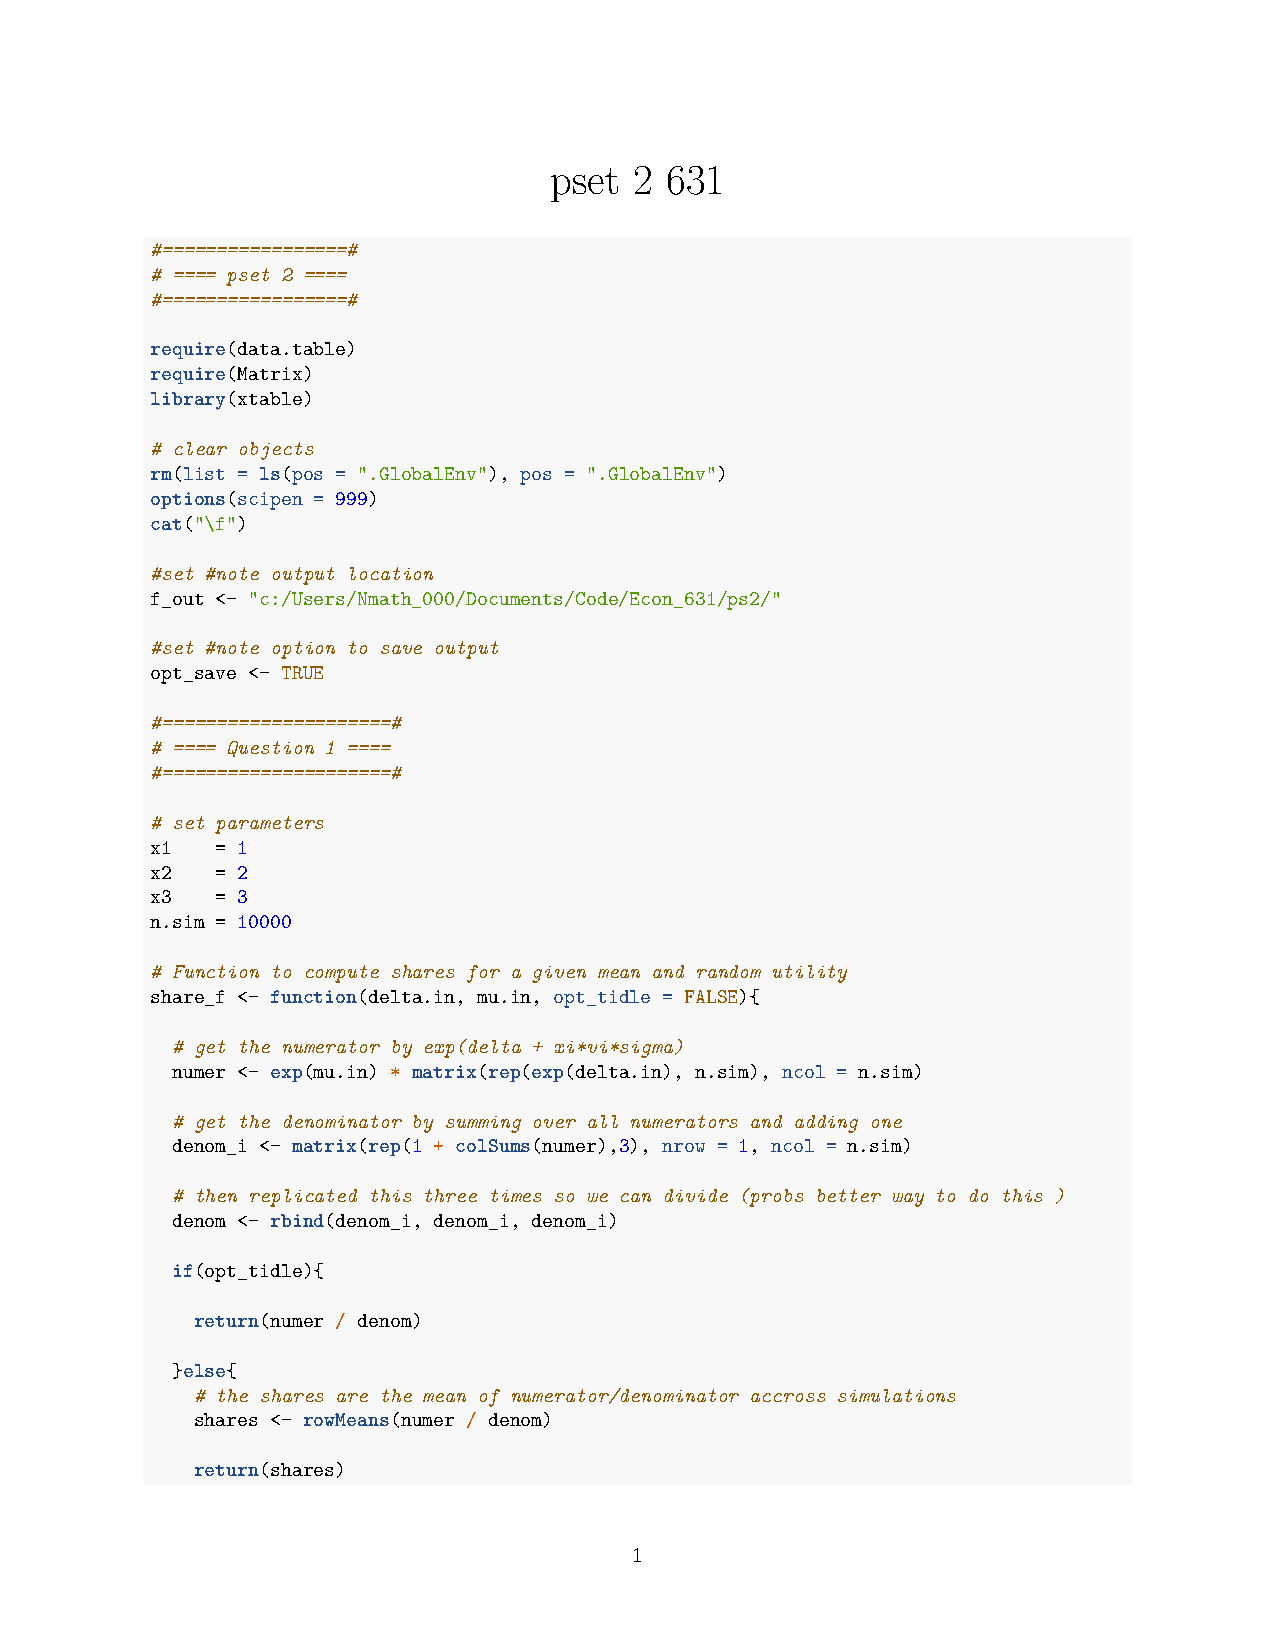
\includepdf[page=-]{assignment_2_r_code_pdf.pdf}





\end{document}
